\documentclass{standalone}
\usepackage{tikz}
\usetikzlibrary{patterns, positioning}


\begin{document}
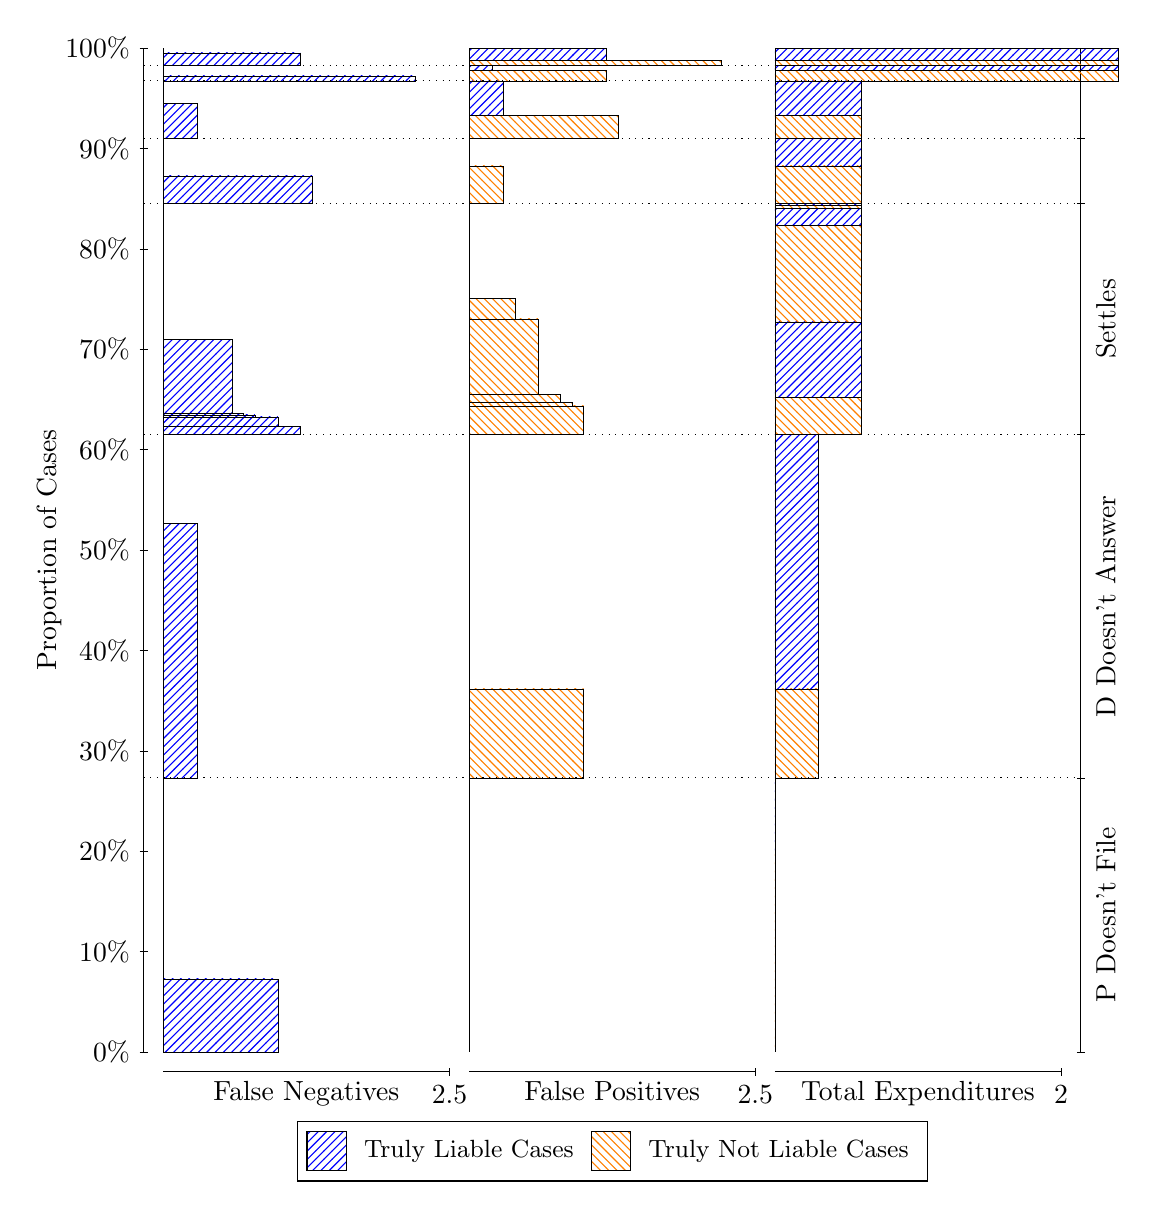
\begin{tikzpicture}
\draw[black, very thin] (1.5,1.75) -- (1.5,14.5);
\node[rotate=90, text=black, anchor=center] at (0.3, 8.125) {Proportion of Cases};
\draw[black, very thin] (1.45,1.75) -- (1.55,1.75);
\node[text=black, anchor=east] at (1.45, 1.75) {0\%};
\draw[black, very thin] (1.45,3.025) -- (1.55,3.025);
\node[text=black, anchor=east] at (1.45, 3.025) {10\%};
\draw[black, very thin] (1.45,4.3) -- (1.55,4.3);
\node[text=black, anchor=east] at (1.45, 4.3) {20\%};
\draw[black, very thin] (1.45,5.575) -- (1.55,5.575);
\node[text=black, anchor=east] at (1.45, 5.575) {30\%};
\draw[black, very thin] (1.45,6.85) -- (1.55,6.85);
\node[text=black, anchor=east] at (1.45, 6.85) {40\%};
\draw[black, very thin] (1.45,8.125) -- (1.55,8.125);
\node[text=black, anchor=east] at (1.45, 8.125) {50\%};
\draw[black, very thin] (1.45,9.4) -- (1.55,9.4);
\node[text=black, anchor=east] at (1.45, 9.4) {60\%};
\draw[black, very thin] (1.45,10.675) -- (1.55,10.675);
\node[text=black, anchor=east] at (1.45, 10.675) {70\%};
\draw[black, very thin] (1.45,11.95) -- (1.55,11.95);
\node[text=black, anchor=east] at (1.45, 11.95) {80\%};
\draw[black, very thin] (1.45,13.225) -- (1.55,13.225);
\node[text=black, anchor=east] at (1.45, 13.225) {90\%};
\draw[black, very thin] (1.45,14.5) -- (1.55,14.5);
\node[text=black, anchor=east] at (1.45, 14.5) {100\%};

\draw[black, very thin] (13.4,1.75) -- (13.4,14.5);
\draw[black, very thin] (13.35,1.75) -- (13.45,1.75);
\node[anchor=west] at (13.35, 1.75) {};
\draw[black, very thin] (13.35,5.2311) -- (13.45,5.2311);
\node[anchor=west] at (13.35, 5.2311) {};
\draw[black, very thin] (13.35,9.5917) -- (13.45,9.5917);
\node[anchor=west] at (13.35, 9.5917) {};
\draw[black, very thin] (13.35,12.528) -- (13.45,12.528);
\node[anchor=west] at (13.35, 12.528) {};
\draw[black, very thin] (13.35,13.351) -- (13.45,13.351);
\node[anchor=west] at (13.35, 13.351) {};
\draw[black, very thin] (13.35,14.083) -- (13.45,14.083);
\node[anchor=west] at (13.35, 14.083) {};
\draw[black, very thin] (13.35,14.28) -- (13.45,14.28);
\node[anchor=west] at (13.35, 14.28) {};
\draw[black, very thin] (13.35,14.5) -- (13.45,14.5);
\node[anchor=west] at (13.35, 14.5) {};

\draw[black, very thin, pattern color=blue, pattern=north east lines] (1.75,1.75) rectangle (3.2033,2.6795);
\draw[black, very thin, pattern color=orange, pattern=north west lines] (1.75,2.6795) rectangle (1.75,5.2311);
\draw[black, very thin, pattern color=blue, pattern=north east lines] (1.75,5.2311) rectangle (2.186,8.4619);
\draw[black, very thin, pattern color=orange, pattern=north west lines] (1.75,8.4619) rectangle (1.75,9.5917);
\draw[black, very thin, pattern color=blue, pattern=north east lines] (1.75,9.5917) rectangle (3.494,9.6929);
\draw[black, very thin, pattern color=blue, pattern=north east lines] (1.75,9.6929) rectangle (3.2033,9.8149);
\draw[black, very thin, pattern color=blue, pattern=north east lines] (1.75,9.8149) rectangle (2.9127,9.8404);
\draw[black, very thin, pattern color=blue, pattern=north east lines] (1.75,9.8404) rectangle (2.7673,9.8619);
\draw[black, very thin, pattern color=blue, pattern=north east lines] (1.75,9.8619) rectangle (2.622,10.796);
\draw[black, very thin, pattern color=orange, pattern=north west lines] (1.75,10.796) rectangle (1.75,12.528);
\draw[black, very thin, pattern color=blue, pattern=north east lines] (1.75,12.528) rectangle (3.6393,12.876);
\draw[black, very thin, pattern color=orange, pattern=north west lines] (1.75,12.876) rectangle (1.75,13.351);
\draw[black, very thin, pattern color=blue, pattern=north east lines] (1.75,13.351) rectangle (2.186,13.794);
\draw[black, very thin, pattern color=orange, pattern=north west lines] (1.75,13.794) rectangle (1.75,14.083);
\draw[black, very thin, pattern color=blue, pattern=north east lines] (1.75,14.083) rectangle (4.9473,14.145);
\draw[black, very thin, pattern color=orange, pattern=north west lines] (1.75,14.145) rectangle (1.75,14.28);
\draw[black, very thin, pattern color=blue, pattern=north east lines] (1.75,14.28) rectangle (3.494,14.438);
\draw[black, very thin, pattern color=orange, pattern=north west lines] (1.75,14.438) rectangle (1.75,14.5);
\draw[black, very thin, pattern color=orange, pattern=north west lines] (5.6333,1.75) rectangle (5.6333,4.3015);
\draw[black, very thin, pattern color=blue, pattern=north east lines] (5.6333,4.3015) rectangle (5.6333,5.2311);
\draw[black, very thin, pattern color=orange, pattern=north west lines] (5.6333,5.2311) rectangle (7.0867,6.3608);
\draw[black, very thin, pattern color=blue, pattern=north east lines] (5.6333,6.3608) rectangle (5.6333,9.5917);
\draw[black, very thin, pattern color=orange, pattern=north west lines] (5.6333,9.5917) rectangle (7.0867,9.9565);
\draw[black, very thin, pattern color=orange, pattern=north west lines] (5.6333,9.9565) rectangle (6.9413,9.995);
\draw[black, very thin, pattern color=orange, pattern=north west lines] (5.6333,9.995) rectangle (6.796,10.101);
\draw[black, very thin, pattern color=orange, pattern=north west lines] (5.6333,10.101) rectangle (6.5053,11.059);
\draw[black, very thin, pattern color=orange, pattern=north west lines] (5.6333,11.059) rectangle (6.2147,11.324);
\draw[black, very thin, pattern color=blue, pattern=north east lines] (5.6333,11.324) rectangle (5.6333,12.528);
\draw[black, very thin, pattern color=orange, pattern=north west lines] (5.6333,12.528) rectangle (6.0693,13.004);
\draw[black, very thin, pattern color=blue, pattern=north east lines] (5.6333,13.004) rectangle (5.6333,13.351);
\draw[black, very thin, pattern color=orange, pattern=north west lines] (5.6333,13.351) rectangle (7.5227,13.64);
\draw[black, very thin, pattern color=blue, pattern=north east lines] (5.6333,13.64) rectangle (6.0693,14.083);
\draw[black, very thin, pattern color=orange, pattern=north west lines] (5.6333,14.083) rectangle (7.3773,14.218);
\draw[black, very thin, pattern color=blue, pattern=north east lines] (5.6333,14.218) rectangle (5.924,14.28);
\draw[black, very thin, pattern color=orange, pattern=north west lines] (5.6333,14.28) rectangle (8.8307,14.342);
\draw[black, very thin, pattern color=blue, pattern=north east lines] (5.6333,14.342) rectangle (7.3773,14.5);
\draw[black, very thin, pattern color=orange, pattern=north west lines] (9.5167,1.75) rectangle (9.5167,4.3015);
\draw[black, very thin, pattern color=blue, pattern=north east lines] (9.5167,4.3015) rectangle (9.5167,5.2311);
\draw[black, very thin, pattern color=orange, pattern=north west lines] (9.5167,5.2311) rectangle (10.062,6.3608);
\draw[black, very thin, pattern color=blue, pattern=north east lines] (9.5167,6.3608) rectangle (10.062,9.5917);
\draw[black, very thin, pattern color=orange, pattern=north west lines] (9.5167,9.5917) rectangle (10.607,10.063);
\draw[black, very thin, pattern color=blue, pattern=north east lines] (9.5167,10.063) rectangle (10.607,11.022);
\draw[black, very thin, pattern color=orange, pattern=north west lines] (9.5167,11.022) rectangle (10.607,12.245);
\draw[black, very thin, pattern color=blue, pattern=north east lines] (9.5167,12.245) rectangle (10.607,12.468);
\draw[black, very thin, pattern color=orange, pattern=north west lines] (9.5167,12.468) rectangle (10.607,12.507);
\draw[black, very thin, pattern color=blue, pattern=north east lines] (9.5167,12.507) rectangle (10.607,12.528);
\draw[black, very thin, pattern color=orange, pattern=north west lines] (9.5167,12.528) rectangle (10.607,13.004);
\draw[black, very thin, pattern color=blue, pattern=north east lines] (9.5167,13.004) rectangle (10.607,13.351);
\draw[black, very thin, pattern color=orange, pattern=north west lines] (9.5167,13.351) rectangle (10.607,13.64);
\draw[black, very thin, pattern color=blue, pattern=north east lines] (9.5167,13.64) rectangle (10.607,14.083);
\draw[black, very thin, pattern color=orange, pattern=north west lines] (9.5167,14.083) rectangle (13.877,14.218);
\draw[black, very thin, pattern color=blue, pattern=north east lines] (9.5167,14.218) rectangle (13.877,14.28);
\draw[black, very thin, pattern color=orange, pattern=north west lines] (9.5167,14.28) rectangle (13.877,14.342);
\draw[black, very thin, pattern color=blue, pattern=north east lines] (9.5167,14.342) rectangle (13.877,14.5);
\draw[black, dotted] (1.5,5.2311) -- (13.4,5.2311);
\draw[black, dotted] (1.5,9.5917) -- (13.4,9.5917);
\draw[black, dotted] (1.5,12.528) -- (13.4,12.528);
\draw[black, dotted] (1.5,13.351) -- (13.4,13.351);
\draw[black, dotted] (1.5,14.083) -- (13.4,14.083);
\draw[black, dotted] (1.5,14.28) -- (13.4,14.28);
\draw[black, very thin] (1.75,1.5) -- (5.3833,1.5);
\node[text=black, anchor=north] at (3.5667, 1.5) {False Negatives};
\draw[black, very thin] (5.3833,1.45) -- (5.3833,1.55);
\node[text=black, anchor=north] at (5.3833, 1.45) {2.5};

\draw[black, very thin] (5.6333,1.5) -- (9.2667,1.5);
\node[text=black, anchor=north] at (7.45, 1.5) {False Positives};
\draw[black, very thin] (9.2667,1.45) -- (9.2667,1.55);
\node[text=black, anchor=north] at (9.2667, 1.45) {2.5};

\draw[black, very thin] (9.5167,1.5) -- (13.15,1.5);
\node[text=black, anchor=north] at (11.333, 1.5) {Total Expenditures};
\draw[black, very thin] (13.15,1.45) -- (13.15,1.55);
\node[text=black, anchor=north] at (13.15, 1.45) {2};

\node[text=black, centered, rotate=90] at (13.72, 3.4905) {P Doesn't File};
\node[text=black, centered, rotate=90] at (13.72, 7.4114) {D Doesn't Answer};
\node[text=black, centered, rotate=90] at (13.72, 11.06) {Settles};





\draw (7.449999999999999,1.5) node[draw=none] (baseCoordinate) {};
\begin{scope}[align=center]
        \matrix[scale=0.5, draw=black, below=0.5cm of baseCoordinate, nodes={draw}, column sep=0.1cm]{
            \node[rectangle, draw, minimum width=0.5cm, minimum height=0.5cm, pattern color=blue, pattern=north east lines] {}; &
            \node[draw=none, font=\small, text=black] (B) {Truly Liable Cases}; &
            \node[rectangle, draw, minimum width=0.5cm, minimum height=0.5cm, pattern color=orange, pattern=north west lines] {}; &
            \node[draw=none, font=\small, text=black] (B) {Truly Not Liable Cases}; \\
            };
\end{scope}

\end{tikzpicture}
\end{document}